\FloatBarrier

{\color{red} 

\section{Toy Generation Method Comparison}\label{app:sampling_vs_reweighting}
During the Run 1-9c analysis the Asimov and data p-values (see sections \ref{sec:sensitivity} and \ref{sec:results}, respectively) were compared to those produced by the P-theta group and differences of $<\SI{0.1}{\sigma}$ were found. It was suggested that these differences may have been due to the different toy generation methods used by VALOR and P-theta. The equivalence of the two methods is assessed in this section.

In this analysis, toys are generated according to the procedure detailed in section \ref{sec:method}, where toys are accepted/rejected based on the likelihood of the control sample data given the toy. p-values are then calculated using only the accepted toys. This method will be referred to as `MC sampling'. The analysis performed by the P-theta group does not use this accept/reject method, instead all toys are accepted the likelihood of the control sample data given the toy is stored and used as a weight when calculating p-values. This method will be referred to as `re-weighting'.

The p-values produced using these two methods will be directly compared using a single set of 3.5M AsimovA-constrained toys. To generate toys, steps 1-\ref{item:toy_gen_test} of the method from section \ref{sec:method} are used, and all 3.5M toys are accepted. In addition, the control sample likelihood of the Asimov A dataset given the toy is stored as the weight, $w$, for each toy. 

After generating the toys, they are all fluctuated (marginalised) to calculate their rate-only (rate+shape) test statistics. Then, without discarding any toys, each toy is labelled as accepted or rejected using a probability of $\frac{w}{\lambda_{max}}$. Two different p-values are then calculated:
\begin{itemize}
	\item MC sampling p-value using only accepted toys e.g. 
	$p(\text{right-tail}) = 
	\frac{ N^{\text{R}}_{\text{acc.}} } 
	{ N^{\text{R}}_{\text{acc.}} + N^{\text{L}}_{\text{acc.}} }$\\
	where $N^{\text{R}}_{\text{acc.}}$ denotes the number of accepted toys in the right tail
	
	\item Re-weighting p-value using all toys e.g. 
	$p(\text{right-tail}) = \frac{\sum_{i=1}^{N^{\text{R}}_{\text{all}}} w_i}
	{ \sum_{i=1}^{N^{\text{R}}_{\text{all}}} w_i + \sum_{i=1}^{N^{\text{L}}_{\text{all}}} w_i}$
	
	%\item Re-weighting p-value using only accepted toys e.g. 
	%$p(\text{right-tail}) = \frac{\sum_{i=1}^{N^{\text{R}}_{\text{acc.}}} w_i}
	%{ \sum_{i=1}^{N^{\text{R}}_{\text{acc.}}} w_i + \sum_{i=1}^{N^{\text{L}}_{\text{acc.}}} w_i}$
\end{itemize}
%TODO: Do I need to include the re-weighting p-value using only accepted toys? What do you learn by comparing the reweighting p-val using only accepted toys to the other two p-vals?

By comparing the MC sampling p-value to the re-weighting p-value for each analysis and hypothesis, the assumption that the two generation methods are equivalent is tested. 

The test statistic distributions of sampled and re-weighted toys are shown for the rate-only analysis in Fig \ref{fig:sensitivity_rate-only_Run1-9d_sampling_test} and for the rate+shape analysis in Fig \ref{fig:sensitivity_rate+shape_Run1-9d_sampling_test}. The test statistic distributions are in good agreement, with small differences from the low statistics of the set of accepted toys: Out of the 3.5M toys generated, the rate-only analysis accepted 8675 and 9005 toys for $\beta=0$ and $\beta=1$, respectively, while the rate+shape analysis accepted 8669 and 9005 toys for $\beta=0$ and $\beta=1$, respectively. 

The resulting p-values are shown in Tab \ref{tab:sampling_vs_reweighting_pvals}. As all of the re-weighting p-values are within the error range of the MC sampling p-values, the two toy generation methods are considered to be equivalent. 

\begin{figure}
	\centering
	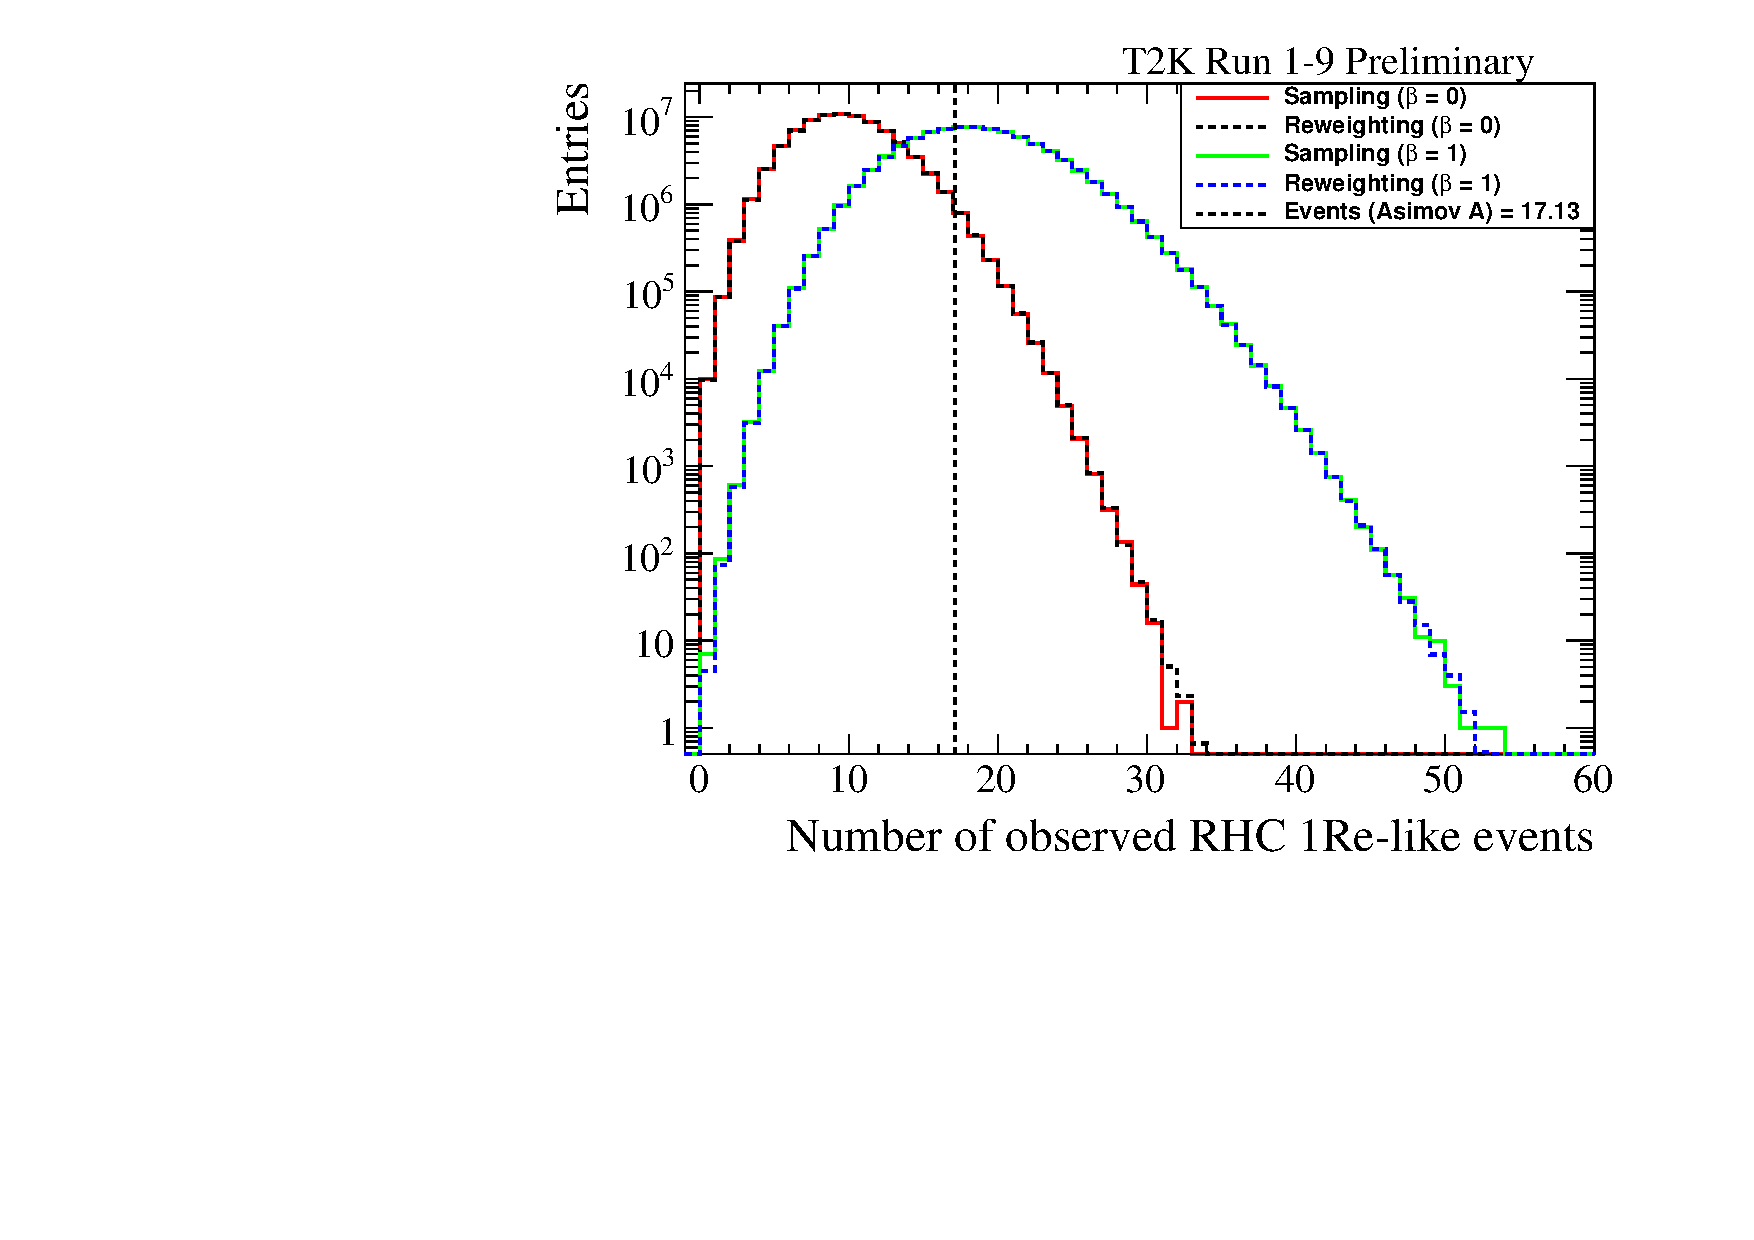
\includegraphics[scale=0.65]{studies/sampling_vs_reweighting/test_sampling_vs_reweighting_rate-only_3500k_Nevents_logscale}
	\caption{Comparison of rate-only test statistic distributions for toy experiments generated by MC sampling and re-weighting. The distribution of the total number of events in the antineutrino mode single-ring e-like sample for both the $\beta = 0$ and $\beta = 1$ hypotheses are produced using full Run 1-9 statistics. The dashed line corresponds to the total number of events given by the Asimov A data set.}
	\label{fig:sensitivity_rate-only_Run1-9d_sampling_test}
\end{figure}

\begin{figure}
	\centering
	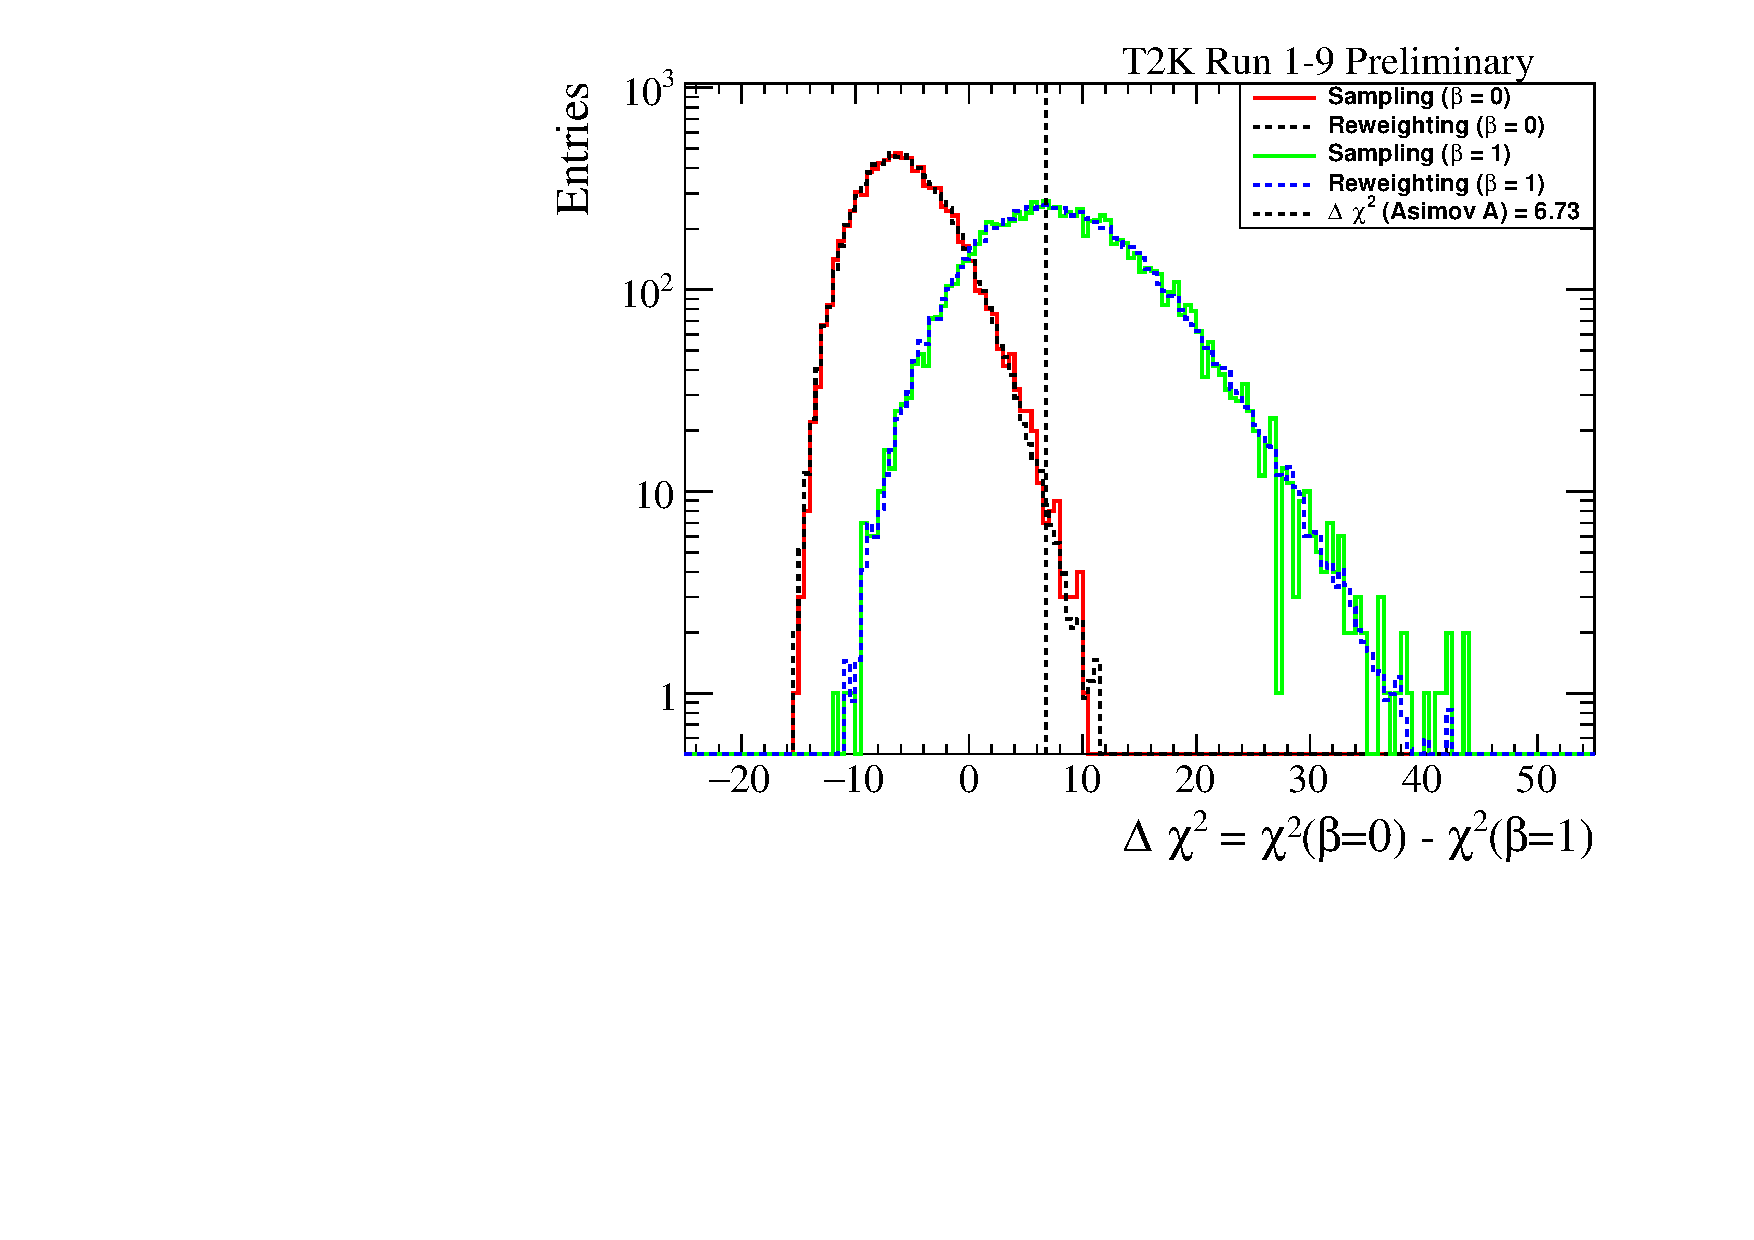
\includegraphics[scale=0.65]{studies/sampling_vs_reweighting/test_sampling_vs_reweighting_rate+shape_3500k_Deltachisq_logscale}
	\caption{Comparison of rate+shape test statistic distributions for toy experiments generated by MC sampling and re-weighting. The distribution of $\Delta \chi^2$ values for both the $\beta = 0$ and $\beta = 1$ hypotheses are produced using full Run 1-9 statistics. The dashed line corresponds to the $\Delta \chi^2$ value given by the Asimov A data set.}
	\label{fig:sensitivity_rate+shape_Run1-9d_sampling_test}
\end{figure}

\begin{table}[H]
\centering
\begin{tabular}{|c|c|c|c|c|}
	\hline
	Analysis                    & Fake data $\beta$   & Toy Gen. Method         & p-value              & $\sigma$               \\
	\hline
	
	
	\multirow{4}{*}{rate-only}  & \multirow{ 2}{*}{0} & MC sampling             & $0.010 \pm 0.001$    & $2.56 \pm 0.04$          \\
	\cline{3-5}
	                            &                     & re-weighting            & $0.01028 \pm 0.00005$& $2.566 \pm 0.002$        \\
	%\cline{3-5}                
	%                           &                     & re-weighting (accepted) & $0.011 \pm 0.001$    & $2.53^{+0.04}_{-0.03}$   \\
	\cline{2-5}
	                            & \multirow{ 2}{*}{1} & MC sampling             & $0.465 \pm 0.005$    & $0.730 \pm 0.009$        \\
	\cline{3-5}
	                            &                     & re-weighting            & $0.4645 \pm 0.0003$  & $0.7315 \pm 0.0004$      \\
	%\cline{3-5}
	%                           &                     & re-weighting (accepted) & $0.482 \pm 0.005$    & $0.703 \pm 0.008$        \\
	\hline
	
	
	\multirow{4}{*}{rate+shape} & \multirow{ 2}{*}{0} & MC sampling             & $0.0040 \pm 0.0007$  & $2.87^{+0.06}_{-0.05}$   \\
	\cline{3-5}
	                            &                     & re-weighting            & $0.0038 \pm 0.0003$  & $2.90 \pm 0.02$          \\
	%\cline{3-5}                
	%                           &                     & re-weighting (accepted) & $0.004 \pm 0.001$    & $2.86^{+0.08}_{-0.07}$   \\
	\cline{2-5}
	                            & \multirow{ 2}{*}{1} & MC sampling             & $0.436 \pm 0.005$    & $0.78 \pm 0.009$         \\
	\cline{3-5}
	                            &                     & re-weighting            & $0.438 \pm 0.002$    & $0.778^{+0.004}_{-0.003}$\\
	%\cline{3-5}
	%                           &                     & re-weighting (accepted) & $0.449 \pm 0.008$    & $0.76 \pm 0.01$          \\
	\hline
	
	
\end{tabular}
\caption{
	Comparison of the p-values obtained using two different toy generation methods, MC sampling and re-weighting.
}
\label{tab:sampling_vs_reweighting_pvals}
\end{table}



} % \colour{red}

\FloatBarrier
